\documentclass{ximera}

%\usepackage{todonotes}

\newcommand{\todo}{}

\usepackage{esint} % for \oiint
\ifxake%%https://math.meta.stackexchange.com/questions/9973/how-do-you-render-a-closed-surface-double-integral
\renewcommand{\oiint}{{\large\bigcirc}\kern-1.56em\iint}
\fi


\graphicspath{
  {./}
  {ximeraTutorial/}
  {basicPhilosophy/}
  {functionsOfSeveralVariables/}
  {normalVectors/}
  {lagrangeMultipliers/}
  {vectorFields/}
  {greensTheorem/}
  {shapeOfThingsToCome/}
  {dotProducts/}
  {partialDerivativesAndTheGradientVector/}
  {../productAndQuotientRules/exercises/}
  {../normalVectors/exercisesParametricPlots/}
  {../continuityOfFunctionsOfSeveralVariables/exercises/}
  {../partialDerivativesAndTheGradientVector/exercises/}
  {../directionalDerivativeAndChainRule/exercises/}
  {../commonCoordinates/exercisesCylindricalCoordinates/}
  {../commonCoordinates/exercisesSphericalCoordinates/}
  {../greensTheorem/exercisesCurlAndLineIntegrals/}
  {../greensTheorem/exercisesDivergenceAndLineIntegrals/}
  {../shapeOfThingsToCome/exercisesDivergenceTheorem/}
  {../greensTheorem/}
  {../shapeOfThingsToCome/}
  {../separableDifferentialEquations/exercises/}
  {vectorFields/}
}

\newcommand{\mooculus}{\textsf{\textbf{MOOC}\textnormal{\textsf{ULUS}}}}

\usepackage{tkz-euclide}
\usepackage{tikz}
\usepackage{tikz-cd}
\usetikzlibrary{arrows}
\tikzset{>=stealth,commutative diagrams/.cd,
  arrow style=tikz,diagrams={>=stealth}} %% cool arrow head
\tikzset{shorten <>/.style={ shorten >=#1, shorten <=#1 } } %% allows shorter vectors

\usetikzlibrary{backgrounds} %% for boxes around graphs
\usetikzlibrary{shapes,positioning}  %% Clouds and stars
\usetikzlibrary{matrix} %% for matrix
\usepgfplotslibrary{polar} %% for polar plots
\usepgfplotslibrary{fillbetween} %% to shade area between curves in TikZ
%\usetkzobj{all}
\usepackage[makeroom]{cancel} %% for strike outs
%\usepackage{mathtools} %% for pretty underbrace % Breaks Ximera
%\usepackage{multicol}
\usepackage{pgffor} %% required for integral for loops



%% http://tex.stackexchange.com/questions/66490/drawing-a-tikz-arc-specifying-the-center
%% Draws beach ball
\tikzset{pics/carc/.style args={#1:#2:#3}{code={\draw[pic actions] (#1:#3) arc(#1:#2:#3);}}}



\usepackage{array}
\setlength{\extrarowheight}{+.1cm}
\newdimen\digitwidth
\settowidth\digitwidth{9}
\def\divrule#1#2{
\noalign{\moveright#1\digitwidth
\vbox{\hrule width#2\digitwidth}}}




% \newcommand{\RR}{\mathbb R}
% \newcommand{\R}{\mathbb R}
% \newcommand{\N}{\mathbb N}
% \newcommand{\Z}{\mathbb Z}

\newcommand{\sagemath}{\textsf{SageMath}}


%\renewcommand{\d}{\,d\!}
%\renewcommand{\d}{\mathop{}\!d}
%\newcommand{\dd}[2][]{\frac{\d #1}{\d #2}}
%\newcommand{\pp}[2][]{\frac{\partial #1}{\partial #2}}
% \renewcommand{\l}{\ell}
%\newcommand{\ddx}{\frac{d}{\d x}}

% \newcommand{\zeroOverZero}{\ensuremath{\boldsymbol{\tfrac{0}{0}}}}
%\newcommand{\inftyOverInfty}{\ensuremath{\boldsymbol{\tfrac{\infty}{\infty}}}}
%\newcommand{\zeroOverInfty}{\ensuremath{\boldsymbol{\tfrac{0}{\infty}}}}
%\newcommand{\zeroTimesInfty}{\ensuremath{\small\boldsymbol{0\cdot \infty}}}
%\newcommand{\inftyMinusInfty}{\ensuremath{\small\boldsymbol{\infty - \infty}}}
%\newcommand{\oneToInfty}{\ensuremath{\boldsymbol{1^\infty}}}
%\newcommand{\zeroToZero}{\ensuremath{\boldsymbol{0^0}}}
%\newcommand{\inftyToZero}{\ensuremath{\boldsymbol{\infty^0}}}



% \newcommand{\numOverZero}{\ensuremath{\boldsymbol{\tfrac{\#}{0}}}}
% \newcommand{\dfn}{\textbf}
% \newcommand{\unit}{\,\mathrm}
% \newcommand{\unit}{\mathop{}\!\mathrm}
% \newcommand{\eval}[1]{\bigg[ #1 \bigg]}
% \newcommand{\seq}[1]{\left( #1 \right)}
% \renewcommand{\epsilon}{\varepsilon}
% \renewcommand{\phi}{\varphi}


% \renewcommand{\iff}{\Leftrightarrow}

% \DeclareMathOperator{\arccot}{arccot}
% \DeclareMathOperator{\arcsec}{arcsec}
% \DeclareMathOperator{\arccsc}{arccsc}
% \DeclareMathOperator{\si}{Si}
% \DeclareMathOperator{\scal}{scal}
% \DeclareMathOperator{\sign}{sign}


%% \newcommand{\tightoverset}[2]{% for arrow vec
%%   \mathop{#2}\limits^{\vbox to -.5ex{\kern-0.75ex\hbox{$#1$}\vss}}}
% \newcommand{\arrowvec}[1]{{\overset{\rightharpoonup}{#1}}}
% \renewcommand{\vec}[1]{\arrowvec{\mathbf{#1}}}
% \renewcommand{\vec}[1]{{\overset{\boldsymbol{\rightharpoonup}}{\mathbf{#1}}}}

% \newcommand{\point}[1]{\left(#1\right)} %this allows \vector{ to be changed to \vector{ with a quick find and replace
% \newcommand{\pt}[1]{\mathbf{#1}} %this allows \vec{ to be changed to \vec{ with a quick find and replace
% \newcommand{\Lim}[2]{\lim_{\point{#1} \to \point{#2}}} %Bart, I changed this to point since I want to use it.  It runs through both of the exercise and exerciseE files in limits section, which is why it was in each document to start with.

% \DeclareMathOperator{\proj}{\mathbf{proj}}
% \newcommand{\veci}{{\boldsymbol{\hat{\imath}}}}
% \newcommand{\vecj}{{\boldsymbol{\hat{\jmath}}}}
% \newcommand{\veck}{{\boldsymbol{\hat{k}}}}
% \newcommand{\vecl}{\vec{\boldsymbol{\l}}}
% \newcommand{\uvec}[1]{\mathbf{\hat{#1}}}
% \newcommand{\utan}{\mathbf{\hat{t}}}
% \newcommand{\unormal}{\mathbf{\hat{n}}}
% \newcommand{\ubinormal}{\mathbf{\hat{b}}}

% \newcommand{\dotp}{\bullet}
% \newcommand{\cross}{\boldsymbol\times}
% \newcommand{\grad}{\boldsymbol\nabla}
% \newcommand{\divergence}{\grad\dotp}
% \newcommand{\curl}{\grad\cross}
%\DeclareMathOperator{\divergence}{divergence}
%\DeclareMathOperator{\curl}[1]{\grad\cross #1}
% \newcommand{\lto}{\mathop{\longrightarrow\,}\limits}

% \renewcommand{\bar}{\overline}

\colorlet{textColor}{black}
\colorlet{background}{white}
\colorlet{penColor}{blue!50!black} % Color of a curve in a plot
\colorlet{penColor2}{red!50!black}% Color of a curve in a plot
\colorlet{penColor3}{red!50!blue} % Color of a curve in a plot
\colorlet{penColor4}{green!50!black} % Color of a curve in a plot
\colorlet{penColor5}{orange!80!black} % Color of a curve in a plot
\colorlet{penColor6}{yellow!70!black} % Color of a curve in a plot
\colorlet{fill1}{penColor!20} % Color of fill in a plot
\colorlet{fill2}{penColor2!20} % Color of fill in a plot
\colorlet{fillp}{fill1} % Color of positive area
\colorlet{filln}{penColor2!20} % Color of negative area
\colorlet{fill3}{penColor3!20} % Fill
\colorlet{fill4}{penColor4!20} % Fill
\colorlet{fill5}{penColor5!20} % Fill
\colorlet{gridColor}{gray!50} % Color of grid in a plot

\newcommand{\surfaceColor}{violet}
\newcommand{\surfaceColorTwo}{redyellow}
\newcommand{\sliceColor}{greenyellow}




\pgfmathdeclarefunction{gauss}{2}{% gives gaussian
  \pgfmathparse{1/(#2*sqrt(2*pi))*exp(-((x-#1)^2)/(2*#2^2))}%
}


%%%%%%%%%%%%%
%% Vectors
%%%%%%%%%%%%%

%% Simple horiz vectors
\renewcommand{\vector}[1]{\left\langle #1\right\rangle}


%% %% Complex Horiz Vectors with angle brackets
%% \makeatletter
%% \renewcommand{\vector}[2][ , ]{\left\langle%
%%   \def\nextitem{\def\nextitem{#1}}%
%%   \@for \el:=#2\do{\nextitem\el}\right\rangle%
%% }
%% \makeatother

%% %% Vertical Vectors
%% \def\vector#1{\begin{bmatrix}\vecListA#1,,\end{bmatrix}}
%% \def\vecListA#1,{\if,#1,\else #1\cr \expandafter \vecListA \fi}

%%%%%%%%%%%%%
%% End of vectors
%%%%%%%%%%%%%

%\newcommand{\fullwidth}{}
%\newcommand{\normalwidth}{}



%% makes a snazzy t-chart for evaluating functions
%\newenvironment{tchart}{\rowcolors{2}{}{background!90!textColor}\array}{\endarray}

%%This is to help with formatting on future title pages.
\newenvironment{sectionOutcomes}{}{}



%% Flowchart stuff
%\tikzstyle{startstop} = [rectangle, rounded corners, minimum width=3cm, minimum height=1cm,text centered, draw=black]
%\tikzstyle{question} = [rectangle, minimum width=3cm, minimum height=1cm, text centered, draw=black]
%\tikzstyle{decision} = [trapezium, trapezium left angle=70, trapezium right angle=110, minimum width=3cm, minimum height=1cm, text centered, draw=black]
%\tikzstyle{question} = [rectangle, rounded corners, minimum width=3cm, minimum height=1cm,text centered, draw=black]
%\tikzstyle{process} = [rectangle, minimum width=3cm, minimum height=1cm, text centered, draw=black]
%\tikzstyle{decision} = [trapezium, trapezium left angle=70, trapezium right angle=110, minimum width=3cm, minimum height=1cm, text centered, draw=black]


\title{Trigonometric}

\begin{document}

\begin{abstract}
coordinates to angles
\end{abstract}
\maketitle



We have discovered that not all functions have an inverse.  Only one-to-one functions have inverses.  We have also seen that we can salvage pieces and parts of functions by restricting their domain and range.  This is necessary for trigonometric functions.





\section*{Sine}

The Sine function is defined as the vertical coordinate of a point on the unit circle at a given angle.  The domain represents angles measured counterclockwise from the positive horizontal axis. The value of $sin(\theta)$ is the vertical coordinate of the point on the unit circle at the angle $\theta$. Therefore, the range of sine is $[-1, 1]$.


Graph of $y = sin(\theta)$.

\begin{image}
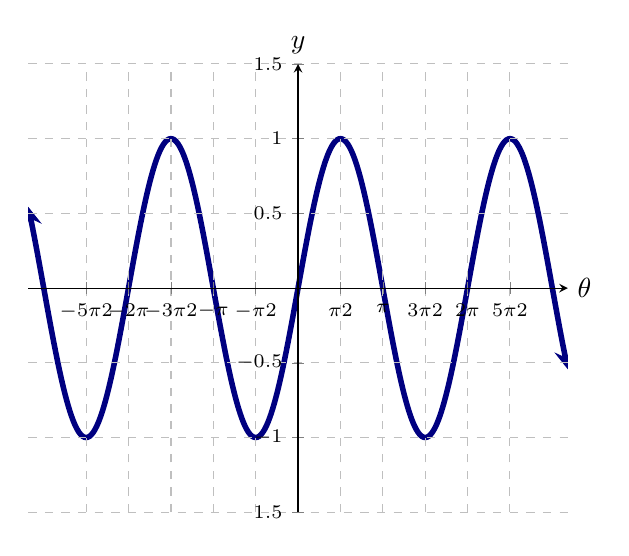
\begin{tikzpicture}
  \begin{axis}[
            domain=-10:10, ymax=1.5, xmax=10, ymin=-1.5, xmin=-10,
            axis lines =center, xlabel={$\theta$}, ylabel=$y$, grid = major, grid style={dashed},
            ytick={-1.5,-1,-0.5,0.5,1,1.5},
            xtick={-7.85, -6.28, -4.71, -3.14, -1.57, 0, 1.57, 3.142, 4.71, 6.28, 7.85},
            xticklabels={$\tfrac{-5\pi}{2}$,$-2\pi$,$\tfrac{-3\pi}{2}$,$-\pi$, $\tfrac{-\pi}{2}$, $0$, $\tfrac{\pi}{2}$, $\pi$, $\tfrac{3\pi}{2}$, $2\pi$, $\tfrac{5\pi}{2}$},
            yticklabels={$1.5$,$-1$,$-0.5$,$0.5$,$1$,$1.5$}, 
            ticklabel style={font=\scriptsize},
            every axis y label/.style={at=(current axis.above origin),anchor=south},
            every axis x label/.style={at=(current axis.right of origin),anchor=west},
            axis on top
          ]
          

            \addplot [line width=2, penColor, smooth,samples=300,domain=(-10:10),<->] {sin(deg(x))};



  \end{axis}
\end{tikzpicture}
\end{image}




The sine function is not one-to-one.  If we want an inverse, then we'll have to restrict the domain.  The most common restriction is $\left[ \frac{\pi}{2}, \frac{\pi}{2} \right]$.




\begin{image}
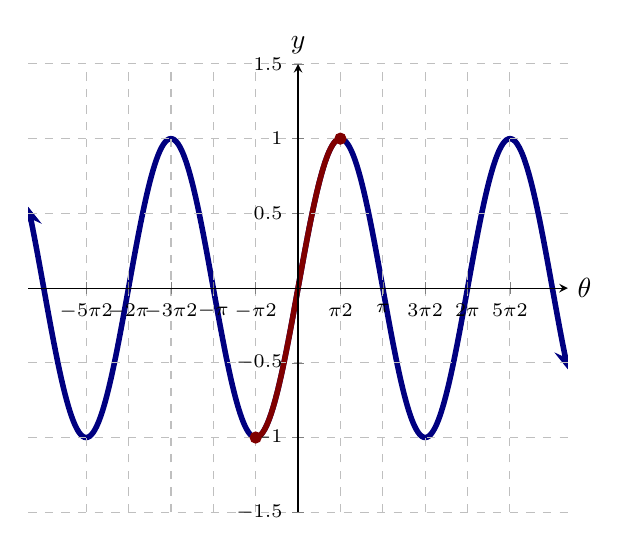
\begin{tikzpicture}
  \begin{axis}[
            domain=-10:10, ymax=1.5, xmax=10, ymin=-1.5, xmin=-10,
            axis lines =center, xlabel={$\theta$}, ylabel=$y$, grid = major, grid style={dashed},
            ytick={-1.5,-1,-0.5,0.5,1,1.5},
            xtick={-7.85, -6.28, -4.71, -3.14, -1.57, 0, 1.57, 3.142, 4.71, 6.28, 7.85},
            xticklabels={$\tfrac{-5\pi}{2}$,$-2\pi$,$\tfrac{-3\pi}{2}$,$-\pi$, $\tfrac{-\pi}{2}$, $0$, $\tfrac{\pi}{2}$, $\pi$, $\tfrac{3\pi}{2}$, $2\pi$, $\tfrac{5\pi}{2}$},
            yticklabels={$-1.5$,$-1$,$-0.5$,$0.5$,$1$,$1.5$}, 
            ticklabel style={font=\scriptsize},
            every axis y label/.style={at=(current axis.above origin),anchor=south},
            every axis x label/.style={at=(current axis.right of origin),anchor=west},
            axis on top
          ]
          

            \addplot [line width=2, penColor, smooth,samples=300,domain=(-10:10),<->] {sin(deg(x))};

            \addplot [line width=2, penColor2, smooth,samples=300,domain=(-1.57:1.57)] {sin(deg(x))};
            \addplot[color=penColor2,fill=penColor2,only marks,mark=*] coordinates{(-1.57,-1)}; 
            \addplot[color=penColor2,fill=penColor2,only marks,mark=*] coordinates{(1.57,1)};



  \end{axis}
\end{tikzpicture}
\end{image}




With this restriction, the inverse of sine is called \textbf{arcsine}, abbreviated \textbf{arcsin}.  




\begin{definition} \textbf{\textcolor{green!50!black}{The Inverse Function of Sine}} 


The inverse of the sine function is called \textbf{arcsine}.  $arcsin(t)$ is an angle between $\frac{-\pi}{2}$ and $\frac{-\pi}{2}$, such that $sin(arcsin(t)) = t$




\begin{itemize}
\item The domain of arcsine is $[-1, 1]$.  
\item The range of arcsine is $\left[ \frac{-\pi}{2}, \frac{\pi}{2} \right]$.
\end{itemize}


\end{definition}


\textbf{Note:} Of course you can also use the general inverse notation: $sin^{-1}(x)$.



The range of arcsine now represents angles, just as the domain of sine does.







\begin{image}
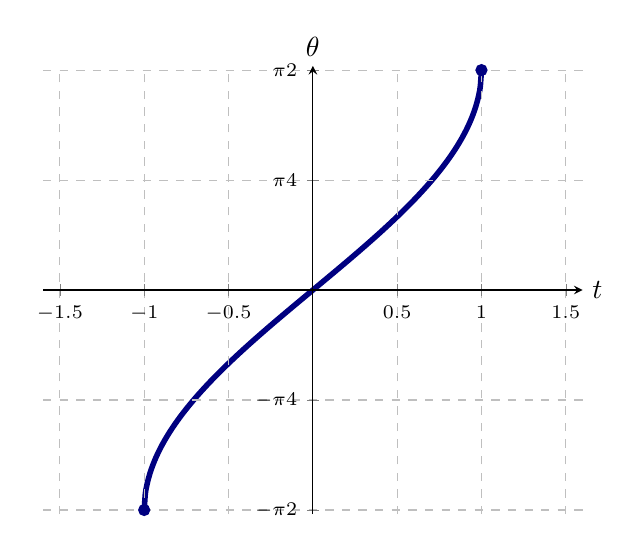
\begin{tikzpicture}
  \begin{axis}[
            domain=-1.6:1.6, ymax=1.6, xmax=1.6, ymin=-1.6, xmin=-1.6,
            axis lines =center, xlabel=$t$, ylabel={$\theta$}, grid = major, grid style={dashed},
            ytick={-1.57, -0.785, 0, 0.785, 1.57},
            xtick={-1.5,-1,-0.5,0.5,1,1.5},
            yticklabels={$\tfrac{-\pi}{2}$, $\tfrac{-\pi}{4}$, $0$, $\tfrac{\pi}{4}$, $\tfrac{\pi}{2}$},
            xticklabels={$-1.5$,$-1$,$-0.5$,$0.5$,$1$,$1.5$}, 
            ticklabel style={font=\scriptsize},
            every axis y label/.style={at=(current axis.above origin),anchor=south},
            every axis x label/.style={at=(current axis.right of origin),anchor=west},
            axis on top
          ]
          

            \addplot [line width=2, penColor, smooth,samples=300,domain=(-1:1)] {asin(x)*pi/180};
            \addplot[color=penColor,fill=penColor,only marks,mark=*] coordinates{(-1,-1.57)}; 
            \addplot[color=penColor,fill=penColor,only marks,mark=*] coordinates{(1,1.57)};



  \end{axis}
\end{tikzpicture}
\end{image}



Because of this restriction, we must keep track of domains and ranges when sine and arcsine interact.

$\blacktriangleright$  The domain of $\sin(\theta)$ is $(-\infty, \infty)$, and the range is $[-1,1]$. \\


$\blacktriangleright$  The domain of $arcsin(y)$ is $[-1,1]$, and the range is $\left[ -\frac{\pi}{2}, \frac{\pi}{2} \right]$.


\begin{example} sin and arcsin

$\sin\left( \frac{3 \pi}{4} \right) = \frac{1}{\sqrt{2}}$

$arcsin\left( \frac{1}{\sqrt{2}} \right) = \frac{\pi}{4} $

\end{example}


















\section*{Cosine}

The Cosine function is defined as the horizontal coordinate of a point on the unit circle at a given angle.  The domain represents angles measured counterclockwise from the positive horizontal axis. The value of $cos(\theta)$ is the horizontal coordinate of the point on the unit circle at the angle $\theta$. Therefore, the range of cosine is $[-1, 1]$.


Graph of $y = cos(\theta)$.






\begin{image}
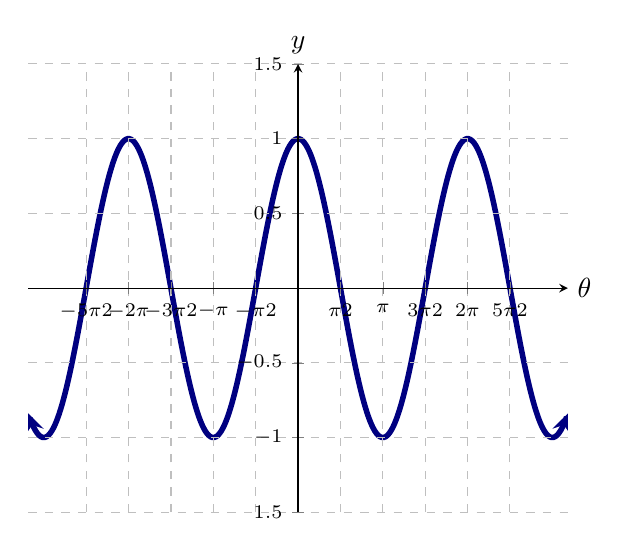
\begin{tikzpicture}
  \begin{axis}[
            domain=-10:10, ymax=1.5, xmax=10, ymin=-1.5, xmin=-10,
            axis lines =center, xlabel={$\theta$}, ylabel=$y$, grid = major, grid style={dashed},
            ytick={-1.5,-1,-0.5,0.5,1,1.5},
            xtick={-7.85, -6.28, -4.71, -3.14, -1.57, 0, 1.57, 3.142, 4.71, 6.28, 7.85},
            xticklabels={$\tfrac{-5\pi}{2}$,$-2\pi$,$\tfrac{-3\pi}{2}$,$-\pi$, $\tfrac{-\pi}{2}$, $0$, $\tfrac{\pi}{2}$, $\pi$, $\tfrac{3\pi}{2}$, $2\pi$, $\tfrac{5\pi}{2}$},
            yticklabels={$1.5$,$-1$,$-0.5$,$0.5$,$1$,$1.5$}, 
            ticklabel style={font=\scriptsize},
            every axis y label/.style={at=(current axis.above origin),anchor=south},
            every axis x label/.style={at=(current axis.right of origin),anchor=west},
            axis on top
          ]
          

            \addplot [line width=2, penColor, smooth,samples=300,domain=(-10:10),<->] {cos(deg(x))};



  \end{axis}
\end{tikzpicture}
\end{image}




The cosine function is not one-to-one.  If we want an inverse, then we'll have to restrict the domain.  The most common restriction is $[0, \pi]$.




\begin{image}
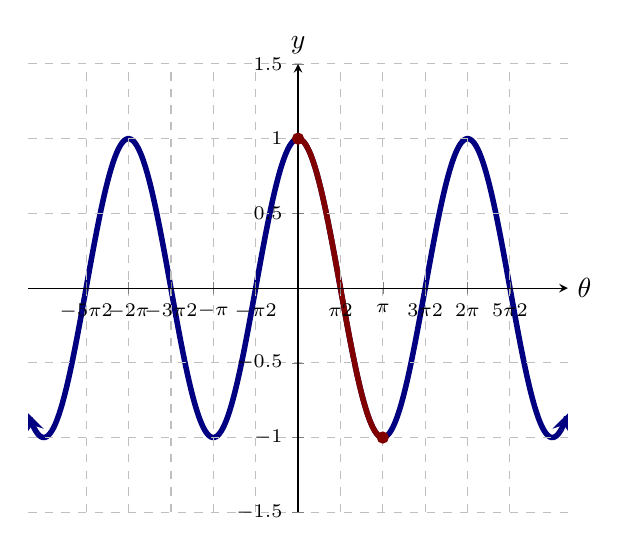
\begin{tikzpicture}
  \begin{axis}[
            domain=-10:10, ymax=1.5, xmax=10, ymin=-1.5, xmin=-10,
            axis lines =center, xlabel={$\theta$}, ylabel=$y$, grid = major, grid style={dashed},
            ytick={-1.5,-1,-0.5,0.5,1,1.5},
            xtick={-7.85, -6.28, -4.71, -3.14, -1.57, 0, 1.57, 3.142, 4.71, 6.28, 7.85},
            xticklabels={$\tfrac{-5\pi}{2}$,$-2\pi$,$\tfrac{-3\pi}{2}$,$-\pi$, $\tfrac{-\pi}{2}$, $0$, $\tfrac{\pi}{2}$, $\pi$, $\tfrac{3\pi}{2}$, $2\pi$, $\tfrac{5\pi}{2}$},
            yticklabels={$-1.5$,$-1$,$-0.5$,$0.5$,$1$,$1.5$}, 
            ticklabel style={font=\scriptsize},
            every axis y label/.style={at=(current axis.above origin),anchor=south},
            every axis x label/.style={at=(current axis.right of origin),anchor=west},
            axis on top
          ]
          

            \addplot [line width=2, penColor, smooth,samples=300,domain=(-10:10),<->] {cos(deg(x))};

            \addplot [line width=2, penColor2, smooth,samples=300,domain=(0:3.14)] {cos(deg(x))};
            \addplot[color=penColor2,fill=penColor2,only marks,mark=*] coordinates{(3.14,-1)}; 
            \addplot[color=penColor2,fill=penColor2,only marks,mark=*] coordinates{(0,1)};



  \end{axis}
\end{tikzpicture}
\end{image}




With this restriction, the inverse of cosine is called \textbf{arccosine}, abbreviated \textbf{arccos}.  







\begin{definition} \textbf{\textcolor{green!50!black}{The Inverse Function of Cosine}} 


The inverse of the cosine function is called \textbf{arccosine}.  $arccos(t)$ is an angle between $0$ and $\pi$, such that $cos(arccos(t)) = t$




\begin{itemize}
\item The domain of arccosine is $[-1, 1]$.  
\item The range of arccosine is $[0, \pi]$.
\end{itemize}


\end{definition}


\textbf{Note:} Of course you can also use the general inverse notation: $cos^{-1}(x)$.




The range of arccos now represents angles, just as the domain of cosine does.










\begin{image}
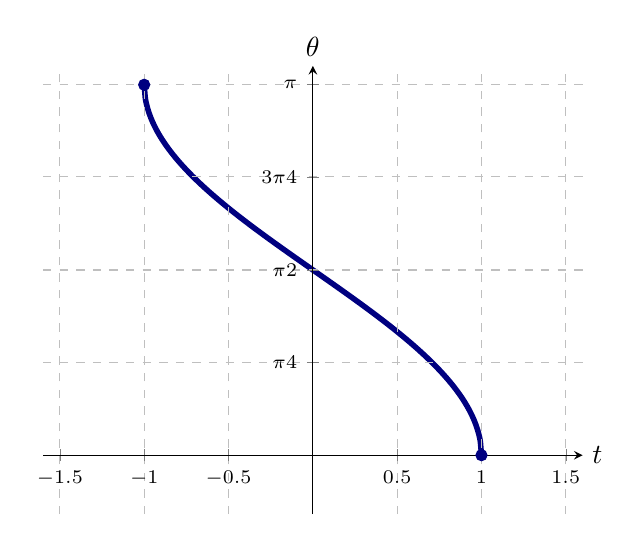
\begin{tikzpicture}
  \begin{axis}[
            domain=-1.6:1.6, ymax=3.3, xmax=1.6, ymin=-0.5, xmin=-1.6,
            axis lines =center, xlabel=$t$, ylabel={$\theta$}, grid = major, grid style={dashed},
            ytick={0, 0.785, 1.57, 2.36, 3.14},
            xtick={-1.5,-1,-0.5,0.5,1,1.5},
            yticklabels={$0$, $\tfrac{\pi}{4}$, $\tfrac{\pi}{2}$, $\tfrac{3\pi}{4}$, $\pi$},
            xticklabels={$-1.5$,$-1$,$-0.5$,$0.5$,$1$,$1.5$}, 
            ticklabel style={font=\scriptsize},
            every axis y label/.style={at=(current axis.above origin),anchor=south},
            every axis x label/.style={at=(current axis.right of origin),anchor=west},
            axis on top
          ]
          

            \addplot [line width=2, penColor, smooth,samples=300,domain=(-1:1)] {acos(x)*pi/180};
            \addplot[color=penColor,fill=penColor,only marks,mark=*] coordinates{(-1,3.14)}; 
            \addplot[color=penColor,fill=penColor,only marks,mark=*] coordinates{(1,0)};



  \end{axis}
\end{tikzpicture}
\end{image}






Because of this restriction, we must keep track of domains and ranges when cosine and arccosine interact.

$\blacktriangleright$  The domain of $\cos(\theta)$ is $(-\infty, \infty)$ and the range is $[-1,1]$. \\


$\blacktriangleright$  The domain of $arccos(y)$ is $[-1,1]$, but the range is $[ 0, \pi ]$.


\begin{example} cos and arccos

$\cos\left( \frac{5 \pi}{4} \right) = -\frac{1}{\sqrt{2}}$

$arccos\left( -\frac{1}{\sqrt{2}} \right) = \frac{3 \pi}{4} $

\end{example}







\section*{Tangent}






\begin{image}
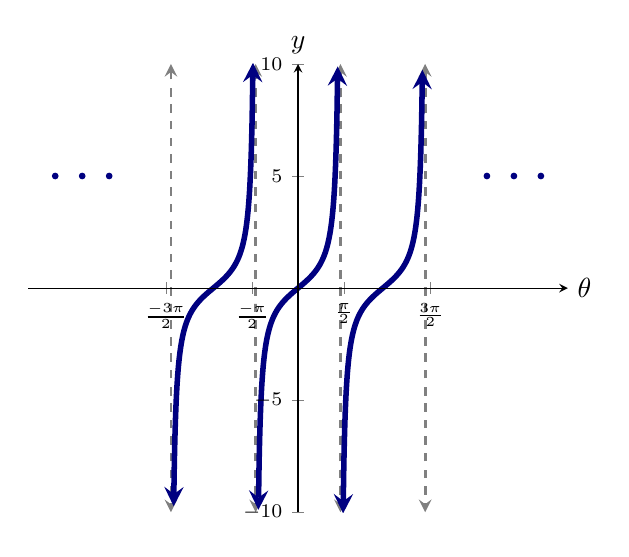
\begin{tikzpicture} 
  \begin{axis}[
            domain=-10:10, ymax=10, xmax=10, ymin=-10, xmin=-10,
            xtick={-4.9, -1.7, 1.7, 4.9}, 
            xticklabels={$\frac{-3\pi}{2}$, $\frac{-\pi}{2}$, $\frac{\pi}{2}$, $\frac{3\pi}{2}$},
            ticklabel style={font=\scriptsize},
            axis lines =center,  xlabel={$\theta$}, ylabel=$y$,
            every axis y label/.style={at=(current axis.above origin),anchor=south},
            every axis x label/.style={at=(current axis.right of origin),anchor=west},
            axis on top
          ]

            \addplot [line width=1, gray, dashed,samples=100,domain=(-10:10), <->] ({-4.71},{x});
            \addplot [line width=1, gray, dashed,samples=100,domain=(-10:10), <->] ({-1.57},{x});
            \addplot [line width=1, gray, dashed,samples=100,domain=(-10:10), <->] ({1.57},{x});
            \addplot [line width=1, gray, dashed,samples=100,domain=(-10:10), <->] ({4.71},{x});

            \addplot [line width=2, penColor, smooth,samples=100,domain=(-1.47:1.47), <->] {tan(deg(x))};
            \addplot [line width=2, penColor, smooth,samples=100,domain=(-4.61:-1.67), <->] {tan(deg(x))};
            \addplot [line width=2, penColor, smooth,samples=100,domain=(1.67:4.61), <->] {tan(deg(x))};

            \addplot[color=penColor,fill=penColor,only marks, mark size=1pt, mark=*] coordinates{(-9,5) (-8,5) (-7,5) (7,5) (8,5) (9,5)};




           

  \end{axis}
\end{tikzpicture}
\end{image}


Arctangent uses the middle piece on $\left( -\frac{\pi}{2}, \frac{\pi}{2} \right)$.







\begin{image}
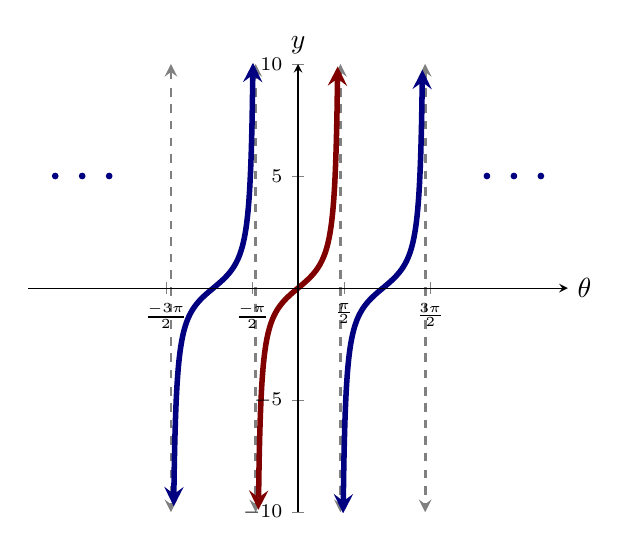
\begin{tikzpicture} 
  \begin{axis}[
            domain=-10:10, ymax=10, xmax=10, ymin=-10, xmin=-10,
            xtick={-4.9, -1.7, 1.7, 4.9}, 
            xticklabels={$\frac{-3\pi}{2}$, $\frac{-\pi}{2}$, $\frac{\pi}{2}$, $\frac{3\pi}{2}$},
            ticklabel style={font=\scriptsize},
            axis lines =center,  xlabel={$\theta$}, ylabel=$y$,
            every axis y label/.style={at=(current axis.above origin),anchor=south},
            every axis x label/.style={at=(current axis.right of origin),anchor=west},
            axis on top
          ]


            \addplot [line width=1, gray, dashed,samples=100,domain=(-10:10), <->] ({-4.71},{x});
            \addplot [line width=1, gray, dashed,samples=100,domain=(-10:10), <->] ({-1.57},{x});
            \addplot [line width=1, gray, dashed,samples=100,domain=(-10:10), <->] ({1.57},{x});
            \addplot [line width=1, gray, dashed,samples=100,domain=(-10:10), <->] ({4.71},{x});

                 
            \addplot [line width=2, penColor2, smooth,samples=100,domain=(-1.47:1.47), <->] {tan(deg(x))};
            \addplot [line width=2, penColor, smooth,samples=100,domain=(-4.61:-1.67), <->] {tan(deg(x))};
            \addplot [line width=2, penColor, smooth,samples=100,domain=(1.67:4.61), <->] {tan(deg(x))};

            \addplot[color=penColor,fill=penColor,only marks, mark size=1pt, mark=*] coordinates{(-9,5) (-8,5) (-7,5) (7,5) (8,5) (9,5)};




           

  \end{axis}
\end{tikzpicture}
\end{image}





With this restriction, the inverse of tangent is called \textbf{arctangent}, abbreviated \textbf{arctan}.  






\begin{definition} \textbf{\textcolor{green!50!black}{The Inverse Function of Tangent}} 


The inverse of the tangent function is called \textbf{arctangent}.  $arctan(t)$ is an angle between $\frac{-\pi}{2}$ and $\frac{-\pi}{2}$, such that $tan(arctan(t)) = t$




\begin{itemize}
\item The domain of arctangent is $(-\infty, \infty)$.  
\item The range of arccosine is $\left( -\frac{\pi}{2}, \frac{\pi}{2} \right)$.
\end{itemize}

\end{definition}


\textbf{Note:} Of course you can also use the general inverse notation: $tan^{-1}(x)$.





The range of arctan now represents angles, just as the domain of tangent does.










\begin{image}
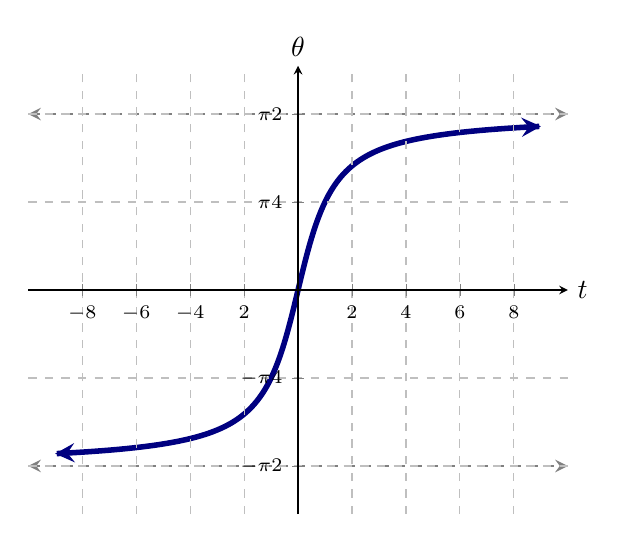
\begin{tikzpicture}
  \begin{axis}[
            domain=-10:10, ymax=2, xmax=10, ymin=-2, xmin=-10,
            axis lines =center, xlabel=$t$, ylabel={$\theta$}, grid = major, grid style={dashed},
            ytick={-1.57, -0.785, 0, 0.785, 1.57},
            xtick={-8,-6,-4,-2,0,2,4,6,8},
            yticklabels={$\tfrac{-\pi}{2}$, $\tfrac{-\pi}{4}$, $0$, $\tfrac{\pi}{4}$, $\tfrac{\pi}{2}$},
            xticklabels={$-8$,$-6$,$-4$,$2$,$0$,$2$,$4$,$6$,$8$}, 
            ticklabel style={font=\scriptsize},
            every axis y label/.style={at=(current axis.above origin),anchor=south},
            every axis x label/.style={at=(current axis.right of origin),anchor=west},
            axis on top
          ]
          

            \addplot [line width=2, penColor, smooth,samples=300,domain=(-9:9),<->] {atan(x)*pi/180};

            \addplot [line width=1, gray, dashed,samples=100,domain=(-10:10), <->] ({x},{1.57});
            \addplot [line width=1, gray, dashed,samples=100,domain=(-10:10), <->] ({x},{-1.57});




  \end{axis}
\end{tikzpicture}
\end{image}

All aspects of a function and its inverse are reversed.

The graph of tangent has vertical asymptotes at $-\frac{\pi}{2}$ and $\frac{\pi}{2}$, therefore, The graph of arctangent has horizontal asymptotes at $-\frac{\pi}{2}$ and $\frac{\pi}{2}$.














\begin{center}
\textbf{\textcolor{green!50!black}{ooooo-=-=-=-ooOoo-=-=-=-ooooo}} \\

more examples can be found by following this link\\ \link[More Examples of Function Algebra]{https://ximera.osu.edu/csccmathematics/precalculus1/precalculus1/functionAlgebra/examples/exampleList}

\end{center}







\end{document}


